\documentclass[12pt,a4paper]{article}
\usepackage[utf8]{inputenc}
\usepackage[german]{babel}
\usepackage[T1]{fontenc}
\usepackage{times}
\usepackage{graphicx}
\usepackage{url}
\usepackage{color}
\usepackage{setspace}
\usepackage{enumerate}
\usepackage{amsmath}
\usepackage{amsfonts}
\usepackage{amssymb}
\usepackage{float}
\usepackage{stix}
\title{Zusammenfassung Theoretische Informatik und Logik}
\author{Henrik Tscherny}
\begin{document}
\maketitle
\tableofcontents

\section{Grundlegende Definitionen}

\subsection{DTM}
$M = (Q,\Sigma,\Gamma,\delta,q_0,F)$
\begin{itemize}
\item $Q$: endliche Zustandsmenge
\item $\Sigma$: Eingabealphabet
\item $\Gamma$: Arbeitsalphabet mit $\Sigma \cup \{\mathvisiblespace \}$
\item $\delta$: Übergangsfunktion (partiell) mit $Q \times \Gamma \rightarrow Q \times \Gamma \times \{L,R,N\}$
\item $q_0$: Startzustand mit $q_0 \in Q$
\item $F$: Menge akzeptierender Endzustände mit $F \subseteq Q$
\end{itemize}

Der Ausdruck $\delta (q,a) = (p, b, D)$ bedeutet:
\begin{itemize}
\item Ist die TM im Zustand q
\item Ließt die TM das Zeichen a
\begin{itemize}
\item wechsele in den Zustand p
\item überschreibe a mit b
\item verschiebe Head nach $D \in \{L,R,N\}$
\end{itemize}
\end{itemize}

\subsection{NTM}
$M = (Q,\Sigma,\Gamma,\delta,q_0,F)$
\begin{itemize}
\item $Q$: endliche Zustandsmenge
\item $\Sigma$: Eingabealphabet
\item $\Gamma$: Arbeitsalphabet mit $\Sigma \cup \{\mathvisiblespace \}$
\item $\delta$: Übergangsfunktion (total) mit $Q \times \Gamma \rightarrow 2^{Q \times \Gamma \times \{L,R,N\}}$
\item $q_0$: Startzustand mit $q_0 \in Q$
\item $F$: Menge akzeptierender Endzustände mit $F \subseteq Q$
\end{itemize}
\flushleft

Anders als bei einer DTM ist die Übergangsfunktion einer NTM mehrdeutig.
Eine NTM akzeptiert sobald mindestens ein Endzustand erreicht werden kann. Dabei werden stets alle möglichen Entscheidungen in $\delta$ betrachtet.
\\
Eine NTM ist genauso berechnungsstark wie eine DTM

\subsection{Church-Turing-These}
\begin{itemize}
\item Jede Funktion die intuitiv berechenbar ist, kann auch von einer TM berechnet werden
\item intuitiv berechenbar meint das es auf irgendeine Weise berechnet werden kann und ist nicht Formal definiert
\item Alle Computer sind gleich (berechnungsstark)
\end{itemize}

\subsection{TM und Funktionen}
\begin{itemize}
\item eine DTM berechnet eine partielle Funktion der Form $f_M: \Sigma^* \rightarrow \Sigma^*$
\item das von der TM berechnete Resultat der Funktion (v) steht nach dem Halten alleinig auf dem Band $w \in \Sigma^*: f_M(w) = v$
\item Funktion undefiniert (darum partiell) bei:
\begin{itemize}
\item M hält auf w aber Bandformat ungültig $\rightarrow$ es steht noch was anderes auf dem Band
\item M hält nicht auf w

\end{itemize}
\item ist $f_M$ total so muss M immer halten
\end{itemize}

\subsection{Berechenbarkeit}
eine Funktion heißt berechenbar, wenn:
\begin{itemize}
\item es gibt eine TM M die f berechnet mit $f = f_M$
\item es gibt einen Algorithmus auf einer TM um das Problem zu lösen
\end{itemize}
Berechenbare totale Funktionen nennt man auch \textbf{rekursiv}\\
Berechenbare partielle Funktionen nennt man auch \textbf{partiell rekursiv}

\subsection{Entscheidbarkeit und Sprachen}
Sei L eine Sprache und M eine TM\\
Sei $L(M)$ die Menge aller Wörter die von einer TM akzeptiert werden d.h. die TM hält in einem Endzustand\\
Sei $w \in L(M)$ das Wortproblem, d.h. ob das Wort w in der Sprache L liegt

\begin{itemize}
\item \textbf{Entscheidbar}: es gibt eine TM die entscheidet ob $w \in L(M)$, M heißt in diesem Fall auch Entscheider
\item \textbf{Semi-Entscheidbar}: die TM verhält sich wie folgt $$
\begin{cases}
w\in L(M) \rightarrow \text{TM hält},\\
w \not\in L(M) \rightarrow \text{TM kann, muss aber nicht halten}\\
\end{cases}
$$
\item \textbf{Co-Semi-Entscheidbar}: Die TM verhält sich umgekehrt zur Semi-Entscheidbarkeit
\item \textbf{Unentscheidbar}: Das Verhalten der TM sagt nichts über das Wortproblem aus
\end{itemize}
Note: andere Objekte können stets als Wörter einer Sprache kodiert werden, daher sollte man die Entscheidbarkeit intuitiv nicht zu eng mit Sprachen in Verbindung bringen
\subsubsection{Sätze}
\begin{itemize}
\item ist L entscheidbar so ist es auch das Komplement von L
\item L ist entscheidbar gdw. L und nicht L ist semi-entscheidbar
\item ist L unentscheidbar und semi-entscheidbar so ist nicht L unentscheidbar und nicht semi-entscheidbar
\end{itemize}

\section{unentscheidbare Probleme}
\subsection{Existenzbeweis}
Folgende Dinge müssen gezeigt werden um die Existenz von unentscheidbaren Problemen zu Beweisen:
\begin{itemize}
\item \textbf{1.} Die Menge der TM's ist abzählbar
\item \textbf{2.} die Menge der Sprachen über jedem Alphabet ist überabzählbar
\end{itemize}
\textbf{1.}
\begin{itemize}
\item Jede TM lässt sich durch ein endliches Wort kodieren, denn jedes Programm besteht aus endlich viel Code ($len(pgrm)\in \mathbb{N}$)
\item alle Wörter sind abzählbar:\\ fange mit $\epsilon$ an, dann alle Wörter mit $len(w) = 1$ dann $len(w) = 2$ usw.
\end{itemize}
\textbf{2.}
\begin{itemize}
\item Nehme an die Menge aller Sprachen wäre abzählbar
\item Erstelle eine große Tabelle welche alle Wörter auf einer Achse aufzählt \textbf{und alle Sprachen auf der anderen*}
\item Markiere in der Tabelle immer ob $w \in L$
\item Konstruiere nun eine neue Sprache $L_d§$ mit $w_i \in L_d \Leftrightarrow w_i \not\in L_i$, d.h. die Sprache $L_d$ entspricht eine Sprache welche sich durch genau einen Eintrag von \textbf{allen} Sprachen unterscheidet
\item es kann sich aber nicht von allen Sprachen unterscheiden, da wir ja davor alle in der Tabelle aufgeschrieben haben \textbf{siehe *}, d.h. \textbf{Widerspruch!}
\item Die Menge aller Sprachen muss überabzählbar sein
\end{itemize}
\subsection{Beispiel $L_{\pi 7}$}
Sei folgendes Problem gegeben
\begin{itemize}
\item Sei $L_{\pi 7}$ die Menge mit Wörtern der Form $7^n$ (Zahl 7, n-mal hintereinander), die in $\pi$ vorkommen 
\item $L_{\pi 7}$ ist entscheidbar, denn:
\begin{itemize}
\item Enthält $\pi$ beliebig lange Siebenerketten, so wird die Sprache Entschieden
\item Enthält $\pi$ nur Siebenerketten bestimmter Länge, so akzeptiere nur für diese Längen
\end{itemize}
\item Für jeden Fall ist ein Algorithmus denkbar
\item aber man weiß nicht welchen
\item das Problem ist entscheidbar aber trotzdem nicht berechenbar
\end{itemize}
\subsection{Beispiel Bussy-Beaver}

Sei eine TM mit leerem Band, n Zuständen und Arbeitsalphabet dem $\Gamma = \{x, \mathvisiblespace \}$\\
Note: es gibt dabei $(2\cdot 2\cdot (n+1))^{2n}$ verschiedene TM's die diese Bedingung erfüllen
\textbf{Frage}:
\begin{itemize}
\item Wie viele Zeichen 'x' kann die TM auf das Band schreiben bevor sie hält
\item die TM muss halten
\item TM's die nicht halten werden ignoriert
\item Sei $BB(n)$ die Anzahl maximal geschriebener Zeichen
\end{itemize}
Note: Alternativ kann man das Problem auch so formulieren: Wie viele Zeichen kann ein beliebiges Python Script ausgeben bevor es sich beendet, wenn das Script gültig ist und das Programm irgendwann terminiert\\
\textbf{Beweis der nicht Berechenbarkeit}
Nehme an BB wäre berechenbar, dann:
\begin{itemize}
\item alle Berechnungen sind dabei unär kodiert, d.h. 4 = 'xxxx' usw.
\item gibt es eine TM $M_{BB}$ die die Funktion $f(n) = BB(n)$ berechnet
\item Sei zudem $M_{+1}$ eine TM mit $f(n) = n+1$ (Inkrementierer)
\item Sei zudem $M_{x2}$ eine TM mit $f(n) = 2n$	(Verdoppler)
\item Sei k die Summe der Anzahl der Zustände in $M_{BB}$, $M_{+1}$ und $M_{x2}$ 
\item Sei $I_k$ eine TM mit $k+1$ Zuständen welche das Wort $x^k$ auf ein leeres Band schreibt
\item Führe $I_k, M_{x2}, M_{BB}, M_{+1}$ hintereinander aus
\item Wir haben somit eine TM mit $\leq 2k$ Zuständen die $BB(2k) +1$ mal 'x' schreibt
\item \textbf{Widerspruch!}: $BB(n)$ sollte ja das Maximum sein wie kann es also noch ein 'x' mehr sein
\item die BB-Funktion ist nicht berechenbar 
\end{itemize}

\subsection{Schwierigkeit von unentscheidbaren Problemen}
\textbf{Existenzbeweis verschieden schwerer unentscheidbarer Probleme}\\
oder: Sind alle unentscheidbaren Probleme auf das Halteproblem Turing-reduzierbar (ex. v. schwereren Prob.)\\
oder: Ist das Halteproblem auf alle unentscheidbaren Probleme Turing-reduzierbar (ex. v. leichteren Prob.)
\begin{itemize}
\item TM's sind endlich beschreibbar
\item Daher gibt es auch nur abzählbar viele TM's
\item Die Menge der Probleme ist aber überabzählbar (siehe Diagonalisierung von Cantor)
\item Eine TM könnte Subroutinen benutzen welche nicht berechenbar sind (z.B. das Halteproblem lösen)
\item Auch solche TM's sind jedoch endlich beschreibbar
\item $\rightarrow$ \textbf{es existieren schwerere Probleme als das Halteproblem}
\end{itemize}
\subsubsection{Beispiele für ein schwereres Problem}
Gegeben sei das Halteproblem höher Ordnung ($P_{HALT}$)
\begin{itemize}
\item eine DTM M welche $P_{HALT}$ als Funktion benutzen darf
\item Frag: Hält M auf w ?
\end{itemize}
Note: Auf diese weise können unendliche viele noch schwerere Probleme konstruiert werden\\
Ein weiteres Problem ist das Universalitätsproblem:
\begin{itemize}
\item Sei eine TM M über $\Sigma$ gegeben
\item akzeptiert die TM alle Eingaben für $w \in \Sigma^*$
\item Es stellt sich heraus, dass dieses Problem auf $P_{HALT}^2$ Turing-reduzierbar ist
\end{itemize} 


\section{Loop}
\subsection{Regeln}
Sei P ein Loop-Programm:
\begin{itemize}
\item alle Variablen sind vom Typ int
\item Wertzuweisung der Form $x := y + n$ für $n\in \mathbb{Z}$
\item For-Schleifen \textbf{LOOP} x \textbf{DO} ... \textbf{END}
\item Programmverkettung: $P_1;P_2$
\item Loop in Loop: \textbf{LOOP} x \textbf{DO} P \textbf{END}
\end{itemize}


\subsection{Eigenschaften}
\begin{itemize}
\item ein Loop-Programm terminiert immer
\item jede Loop-berechenbare Funktion ist total
\item es gibt berechenbare Funktionen die nicht Loop-berechenbar sind (z.B.) Ackermann-Funktion
\item alle kleiner als $O(n^{n^{n^{...^{x}}}})$ laufenden Funktionen sind Loop berechenbar
\end{itemize}
\subsubsection{BB-Funktion für Loop}
Sei $BB_{Loop}$ die eine Funktion die für ein Loop Programm der Länge l, die größte Zahl die ein Loop Programm dieser Länge erzeugen kann, bei leerer Startkonfiguration\\
Wir zeigen 2 Dinge:
\begin{itemize}
\item $BB_{Loop}$ ist berechenbar
\item $BB_{Loop}$ ist nicht Loop-berechenbar
\end{itemize}
\textbf{1.}
\begin{itemize}
\item Es gibt endlich viele Loop Programme der Länge $\leq l$
\item Durch diese kann man in endlicher Zeit durch iterieren
\item gebe am Ende das Maximum zurück
\item ein Loop Programm muss vorher wissen wie viele Schleifendurchläufe benötigt werden, da es dies selbst nicht berechnen kann (diese Aussage könnte jedoch eine TM für das Loop Programm treffen)
\item Loop ist berechnungsschwächer als eine TM
\end{itemize}
\textbf{2.}
\begin{itemize}
\item Annahme, es $BB_{Loop}$ ist Loop-berechenbar
\item Sei k die Länge eines Loop Programms $P_{BB}$ welches $BB_{Loop}$ berechnet
\item Wähle $m \geq k + 17 + log_{10} m$
\item Sei $P_m$ ein Programm welches m zu einer Zahl x addiert (Länge 7)
\item Sei $P_{++}$ ein Programm welches x inkrementiert (Länge 8)
\item Sei $P = P_m;P_{BB};P_{++}$ mit Länge $k + 17 + log_{10} m$
\item P gibt somit $BB_{Loop}(m) + 1$ aus, jedoch ist die Länge von P kürzer als m
\item Widerspruch
\end{itemize}

\section{While}
\subsection{Regeln}
\begin{itemize}
\item jedes Loop Programm ist ein While Programm
\item \textbf{WHILE} condition \textbf{DO} P \textbf{END}
\end{itemize}

\subsection{Eigenschaften}
\begin{itemize}
\item While Programme sind genauso berechnungsstark wie TM's
\item  $\rightarrow$ DTM's können White Programme simulieren
\item $\rightarrow$ While Programme können TM's simulieren
\item While Programme terminieren nicht immer
\item können alle berechenbaren totalen und partiellen Funktionen berechnen
\end{itemize}

\subsection{Universalmachine}
\begin{itemize}
\item TM's sind stark genug andere TM's zu simulieren
\item Die simulierende TM kodiert dabei die andere(n) TM'(s) in ihrem Alphabet (Emulator)
\item Die Universalmachine U simuliert für eingaben der Form $enc(M)\#\#enc(w)$ w auf M$$
\begin{cases}
\text{M hält auf w} \rightarrow \text{U hält auf enc(w)},\\
\text{M hält nicht auf w} \rightarrow \text{U hält nicht auf enc(w)}\\
\end{cases}
$$
\item $\rightarrow$ Universalrechner sind möglich
\item $\rightarrow$ es gibt Software
\end{itemize}

\section{Halteproblem}
\subsection{Definition}
Das Halteproblem ist die Frage:\\
Wird eine TM M auf einem Wort w jemals anhalten ?\\
Formal:\\
$P_{HALT} = \{end(M)\#\# enc(w) | \text{M hält auf w}\}$
\subsection{Beweis der Unentscheidbarkeit}
$P_{HALT}$ ist entscheidbar gdw. es und sein Komplement semi-entscheidbar sind
\begin{itemize}
\item Nehme an das Komplement sei semi-entscheidbar
\item Konstruiere eine TM F wie folgt$$
\begin{cases}
\text{hält} \rightarrow \text{TM hält auf w nicht},\\
\text{hält-nicht} \rightarrow \text{sonst}\\
\end{cases}
$$, diese TM zeigt also immer das genau entgegengesetzte Halteverhalten
\item gebe F in sich selbst ein (F ist Programm und Maschine zugleich)
\item 1. Möglichkeit: F hält auf F nicht, darum müsste F halten, Widerspruch da F halten muss wenn F nicht hält laut Definition
\item 2. Möglichkeit: F hält auf F, darum müsste F nicht halten nach Definition von F, Widerspruch
\item $\rightarrow$ das Halteproblem ist semi-entscheidbar
\end{itemize}

\section{Reduktionen}
Mittels Reduktion können Aussagen bzgl. der relativen Schwierigkeit von Problemen getroffen werden, z.B. A ist mindestens genauso schwierig wie B oder B ist nicht leichter als A
\begin{itemize}
\item Many-One Reduktion kann als Turing-Reduktion ausgedrückt werden
\item es gibt Probleme die Turing aber nicht Many-One reduzierbar sind
\item Bsp. $P_{HALT} \leq_T \bar{P_{HALT}}$ aber nicht $P_{HALT} \leq_m \bar{P_{HALT}}$
\item Turing-Reduktion kann nur Entscheidbarkeit oder Unentscheidbarkeit, nicht aber Semi-Entscheidbarkeit zeigen
\end{itemize}

\subsection{Turing Reduktion}
\begin{itemize}
\item Bei der Turing Reduktion benutzt man ein zwei Programme P und Q
\item P sei auf ein Problem Q Turing reduzierbar ($P \leq_T Q$) wenn man P mittel Q lösen kann
\item sprich, P ist nicht schwerer zu lösen aus Q (kann aber leichter sein)
\item Q ist mindestens so schwer wie P (oder schwerer)
\item lässt sich beispielsweise ein Problem auf das Halteproblem reduzieren, so ist das Problem nicht berechenbar
\item sprich, ist $P \leq_T Q$ und $P=P_{HALT}$ dann 'ist das Halteproblem höchstens so schwierig wie Q' oder 'Q ist mindestens so leicht wie das Halteproblem'
\end{itemize}

\subsection{Many-One Reduktion}
\begin{itemize}
\item Es sind zwei Probleme P und Q gegeben
\item Findet man eine Funktion f mit $w \in P \Leftrightarrow f(w) \in Q$ so ist P auf Q Many-One reduzierbar $P \leq_m Q$
\end{itemize}
Beispiel: Reduktion des Halteproblems auf das $\epsilon$-Halteproblem (Wird M auf $\epsilon$ halten?)
\begin{itemize}
\item Sei M eine TM und eine andere TM $M_w$ wie folgt konstruiert:
\item Lösche Eingabeband und fülle es mit dem Wort w
\item Verarbeite die Eingabe wie M
\item $$ f(v) = 
\begin{cases}
enc(M_w) \rightarrow v=enc(M)\#\#enc(w) \text{für eine TM M},\\
\# \rightarrow \text{ungültige Eingabe}\\
\end{cases}
$$
\item Ist $P \leq_m Q$ und Q ist semi-entscheidbar, dann ist auch P semi-entscheidbar
\end{itemize}
Note: ist f eine in polynomiell Zeit berechnenbare Funktion so ist es eine \textbf{polynomielle Many-One Reduktion} und man schreibt $P \leq_p Q$

\section{Satz von Rice}

\subsection{Definition}
\begin{itemize}
\item Jede nicht-triviale Frage über von einer Turingmaschine ausgeführten Berechnung ist unentscheidbar
\item Sei E einer Eigenschaft von Sprachen, welche für manche (semi)-entscheidbare Sprachen gilt und für manche nicht
\end{itemize}
\subsection{Beweis}
\begin{itemize}
\item Konstruiere eine Many-One Reduktion vom $\epsilon$-Halteproblem auf die 'E-Haltigkeit'
\item Sei $\emptyset \not\in E$
\item Sei $M_L$ eine TM, die eine Sprache $L \in E$ akzeptiert
\item Sei $M^*$ wie folgt: Simuliere das $\epsilon$-Halteproblem und simuliere $M_L$ auf w sofern M hält
\item somit, hält M auf so ist die von $M^*$ erkannte Sprach eine Sprache mit der Eigenschaft E
\item wenn nicht, dann ist die $L(M^*)$ leer und hat nicht die Eigenschaft E
\item $$
\begin{cases}
enc(M^*) \rightarrow v = enc(M) \text{für eine TM M},\\
\# \rightarrow \text{ungültige Eingabe}\\
\end{cases}
$$
\end{itemize}

\section{Postsches-Korrespondenz-Problem (PCP)}
\subsection{Definition und Eigenschaften}
Gegeben ist folgender Sachverhalt:
\begin{itemize}
\item Dominosteine mit Wortpaaren über $\Sigma^*$
\item die Länge der Wörter auf einem Dominostein kann sich unterscheiden
\item Frage: kann man eine Kombination aus gegeben Dominosteinen finden, sodass die beiden Gesamtwörter (also oben und unten) gleich sind?
\item modifizieren des PCP, sodass ein Startsein gegeben ist mit dem man anfangen muss (MPCP)
\item das PCP ist unentscheidbar
\end{itemize}
\subsection{Beweis der Unentscheidbarkeit}
Ziel: Reduzieren des MPCP auf das Halteproblem, und des MPCP auf das PCP\\
\textbf{Konstruktion}\\
\begin{itemize}
\item Nimm eine Instanz des MPCP, d.h. das PCP mit einem gegebenen Startstein
\item Finde dazu eine Many-One Reduktion die das MPCP auf das Halteproblem reduziert (MPCP ist mindestens so schwer wie das Halteproblem)
\item Kodiere das entstehende Lösungswort des MPCP als Abfolge von Konfigurationen (Zustand, Bandinhalt, HEAD-Position) wie folgt:
\begin{itemize}
\item $(vqw)$ sei eine Konfiguration (v = Bandinhalt links, q = HEAD, w = Bandinhalt rechts)
\item Folge von Konfigurationen (Lauf) getrennt mit Trennzeichen ($\#$) $\rightarrow$ ($c_1 \# c_2  \# ...$)
\end{itemize}
\item Lösung ist dann wie folgt:
\begin{itemize}
\item Hält die TM, d.h. ist die Abfolge endlich: es gibt eine Lösung
\item Hält die TM nicht: es gibt keine Lösung
\end{itemize}
\item nehme als Startstein einen welcher oben leer ist und unten bereits eine Konfiguration steht\\
$ \left[ {\# \atop \# c_0 \#} \right]$
\item finde nun Steine die oben das haben was unten gefordert ist
\item dazu benutze die folgenden Regeln und das untere Wort nach oben zu kopieren$$
\begin{cases}
\left[ {qa \atop bp} \right] \rightarrow \delta(q,a) = \langle p,b,R \rangle,\\
\left[ {cqa \atop pcb} \right] \rightarrow \delta(q,a) = \langle p,b,L \rangle \text{und $c \in \Gamma$ beliebig},\\
\left[ {qa \atop pb} \right] \rightarrow \delta(q,a) = \langle q,b,N \rangle\\
\end{cases}
$$
\item zusätzliche Randregeln:$$
\begin{cases}
\left[ {\# qa \atop \# bp} \right] \rightarrow \delta(q, a) = \langle p, b, L \rangle \text{anstoßen am linken Rand},\\
\left[ {q \# \atop q \mathvisiblespace \# } \right] \rightarrow \forall q \in Q \text{unendlich nach rechts}\\
\end{cases}
$$
\item zusätzlich nehmen wir eine Kopierregel welche es erlaubt von unten nach oben zu kopieren:\\
$\left[ {x \atop x} \right] \rightarrow \forall x \in \Gamma \cup \{ \# \}$
\item Startregel:\\
$ \left[ {\# \atop \# q_0 w \#} \right] \text{mit } q_0 = S, w \in \Sigma^*$
\item Zudem definieren wir noch ein weites Symbol $ \$ $ um den Endstein zu markieren:$$
\begin{cases}
\left[ {qa \atop \$} \right] \rightarrow \delta(q, a), \text{undefiniert und } a\in \Gamma,\\
\left[ {a\$ \atop \$} \right], \text{und } \left[ {\$ \atop a\$} \right], \rightarrow \forall a \in \Gamma.\\
\left[ {\$ \# \# \atop \#} \right] \rightarrow \text{endgültiger Abschluss}
\end{cases}
$$
\end{itemize}
\textbf{Beweis}
\begin{itemize}
\item man kann nun eine Abfolge von Konfigurationen finden, welche der Konstruktion folgt:
\item der Ausgang des Laufs, kann das wie folgt interpretiert werden:\\
\begin{itemize}
\item hält: MPCP hat Lösung
\item nicht hält: undefiniert
\end{itemize}
\item Um das MPCP auf das PCP zu reduzieren definieren wir noch 3 Dinge:
\begin{itemize}
\item $_\#w_\#$, Wörter mit Trennzeichen vor und hinter jedem Zeichen
\item $_\#w$, Wörter mit Trennzeichen vor jedem Zeichen
\item $w_\#$, Wörter mit Trennzeichen nach jedem Zeichen
\end{itemize}
\item Sei eine Reduktion nun wie folgt:
\begin{itemize}
\item beginne mit einem Domino mit beidseitigem Trennzeichen oben und nur linksseitigen Trennzeichen unten
$ \left[ { _\#x_{1\#} \atop _\#y_1 } \right]$
\item setze die Kette nun mit Steinen fort, welche oben rechtsseitig und unten linksseitig getrennt sind
$ \left[ { x_{n\#} \atop _\#y_n } \right]$
\item der letzte Stein soll ein spezieller Stein sein
$ \left[ { \$ \atop \# \$ } \right]$
\end{itemize}
\item Besitzt nun das MPCP eine Lösung, so hat das entsprechende PCP auch eine Lösung
\item jedes Symbol ist dabei von einer $\#$ umgeben
\item das Wort endet auf $\$ $
\item Besitzt das PCP eine Lösung, so muss es mit dem ersten Wortpaar beginnen, da nur dies oben und unten eine $ \# $ besitzt
\item lässt man alle $ \# $ und  $ \$ $ weg, so hat man wieder eine Lösung für das MPCP
\item d.h. PCP und MPCP unterscheiden sich nur durch Trennzeichen
\item $\Rightarrow$ \textbf{PCP und MPCP sind semi-entscheidbar}
\end{itemize}
\subsubsection{Beweis Beispiel}
\begin{itemize}
\item gegebene TM:
\begin{figure}[H]
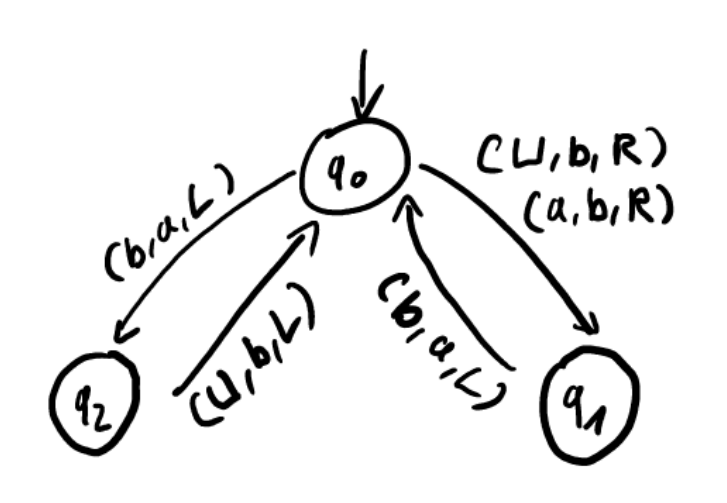
\includegraphics[scale=0.3]{resources/tm1.png}
\caption{gegebene TM}
\label{fig}
\end{figure}
\item Wort w: \textbf{aba}
\item Lässt man die TM nun auf w laufen so erhält man:\\
$\# q_0 aba \# b q_1 ba \# q_0 baa \# q_2 \mathvisiblespace aaa \# q_0 \mathvisiblespace baaa \# b q_1 baaa$ usw.\\
\item Ziel: das erzeugte Resultat oben und unten auf den Steinen
\item dazu nutzte die Regeln von Oben
\item $\left[ {\# \atop \# q_0 aba \#} \right] \rightarrow \left[ {\# \atop \# q_0 aba \#} \right] \left[ {q_0 a \atop b q_1} \right]$
\item Regel 1: in $q_0$ lese a $\rightarrow$ gehe in $q_1$ schreibe b
\item nutze Regeln bis oben=unten
\end{itemize}

\newpage
\section{Komplexität}
\subsection{asymptotische Laufzeit}
Note: alles gesagte ist äquivalent auf Speicherbedarf (benutzte Speicherzellen) übertragbar\\
\textbf{O-Notation}
\begin{itemize}
\item sei $f, g: \mathbb{N} \rightarrow \mathbb{R}$ und $f \in O(g)$
\item nehme eine Zahl $c > 0$ (Konstante) und ein $n_0 \in \mathbb{N}$ (untere Schranke)
\item gilt $n > n_0$ und $f(n) \leq c\cdot g(n)$ wächst f nicht wesentlich schneller als g
\item d.h. f unterscheidet sich von g nicht mehr als um einen linearen Teil
\item Sei: $f: 2x^2$ und $g:x^2+10$
\begin{itemize}
\item beide Funktionen steigen etwa quadratisch
\item f  unterscheidet sich von g um den Faktor 2x, dies ist aber im Rahmen (Konstante c>0)
\item und $f \geq g$ für ein $n_0$, also der Schnittpunkt der Parabeln
\item die Notation versteckt absolute Anteile (Konstanten) (z.B.) $10n^3 = O(n^3)$
\end{itemize}
\item Trotz kleiner O-Notation kann der tatsächliche Wert trotzdem extrem abweichen da der Grenzwert betrachtet wird
\begin{itemize}
\item $2^n + n^{2000} \in O(2^n)$
\item $2^{1000} \in O(1)$
\item $4^n \in O(2^n)$
\item $x^2 > 2^n$ für $n \in [2, 4]$,\hspace{5pt} (aber $(O(2^n) > O(n^2)$), siehe Abb.2
\end{itemize}
\end{itemize}
\begin{figure}[H]
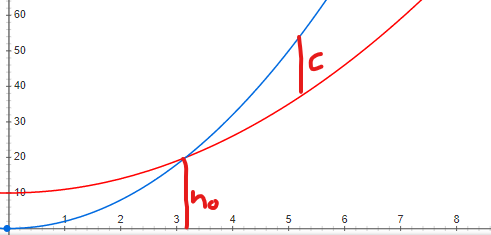
\includegraphics[scale=0.6]{resources/O-vergleich.png}
\caption{Veranschaulichung von f, g, sowie c und $n_0$}
\label{fig}
\end{figure}
\textbf{andere Laufzeiten}\\
\begin{figure}[H]
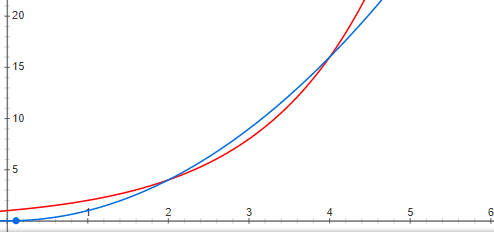
\includegraphics[scale=0.6]{resources/exp_vs_poly.png}
\caption{Vergleich von $x^2$ und $2^x$}
\label{fig}
\end{figure}
\textbf{andere Laufzeiten}\\
\hfill

\begin{tabular}{|c|c|c|}
\hline
Notation & $ C = \lim_{n\rightarrow \infty} \frac{f(n)}{g(n)}$ & Bedeutung \\
\hline
$f \in O(g)$ & $c < 0$ & $f\leq g$\\
\hline
$f \in \Omega(g)$ & $c >0$ & $f\geq g$\\
\hline
$f \in \Theta(g)$ & $0<c<\infty$ & $f=g$\\
\hline
$f \in o(g)$ & $c=0$ & $f<g$\\
\hline
$f \in \omega(g)$ & $c=\infty$ & $f>g$\\
\hline
\end{tabular}
\subsection{Linear Speedup Theorem}
\textbf{Definition}\\
\begin{itemize}
\item Sei M eine multiband-TM mit k Bändern
\item M hält bei einer Eingabe der Länge n nach f(n) Schritten
\item Es gibt eine k-Band TM' die nach maximal  $\frac{f(n)}{c} +n + 2$ Schritten hält für jedes $c > 0, c\in \mathbb{N}$
\item (n+2) Kodierungsoverhead $\rightarrow$ n ... einmal über den Speicher iterieren, 2 ... Feststellen des Endes
\item sprich, Jede Turingmaschine kann um einen linearen Faktor beschleunigt werden
\item möglich durch Zusammenfassen von Speicherzellen zu einer, durch das benutzen eines unendlichen (sehr großen) Bandalphabets (Bandkompression)
\item man benutzt quasi eine riesige Look-up-table über alles was passieren kann
\item Problem: reale Rechner können kein unendliches Arbeitsalphabets benutzen, sondern nur $\{0, 1\}$
\item Problem 2: in der Praxis kann man nicht beliebig große Daten in einem Schritt lesen
\item Problem 3: Linearer Speedup ist immer noch relativ klein $O(n)$
\end{itemize}
\textbf{Beweis}\\
\begin{itemize}
\item vergrößere das Bandalphabet von M': $\Gamma ' = \Sigma \cup \Gamma^{6c}$ (6c-große Tupel)
\item möchte man z.B. einen Speedup von 1000-x so müssen 6000 Zeichen an einer Bandposition kodiert werden
\item M' kodiert nun 6c Zeichen des Eingabebandes und schreibt ein Zeichen aus $\Gamma^{6c}$ auf Band 2
\item nun simuliere M
\begin{itemize}
\item lese das Band von den jetzigen Positionen der k-Bänder und Rechts und Links davon (benötigt 4 Schritte)
\item Speichere das gelesene wird als Zustand gespeichert es gibt somit $|Q \times \{1,...,k\}^{18ck}|$ Zustände
\item dieser Zustand enthält nun die gelesenen Information vom TM-Head sowie rechts und links davon, aber als ein Zustand
\item Simuliere nun in 2 Schritten die nächsten 6c Schritte von M
\end{itemize}
\item Simulation von 6c M-Schritten in 6 M'-Schritten
\end{itemize}

\subsection{Komplexitätsklassen}
\textbf{Definitionen}\\
Sei f(n) Eine obere Schranke von Einheiten einer Resource welche benutzt werden können, bei einer Eingabe der Länge n, dann:\\
\begin{itemize}
\item Sei $DTIME(f(n))$ die Klasse aller Sprachen L, welche durch eine $O(f)$ zeitbeschränkte \textbf{DTM} entschieden werden können
\item Sei $DSPACE(f(n))$ analog zum Speicher
\item Sei $NTIMEf(n))$ die Klasse aller Sprachen L, welche durch eine $O(f)$ zeitbeschränkte \textbf{NTM} entschieden werden können
\item Sei $NSPACE(f(n))$ analog zum Speicher
\end{itemize}
\textbf{Eigenschaften}
\begin{itemize}
\item Verschiedene Modelle von DTM's (z.B. Mehrband-TM, WHILE, etc.) resultieren in verschiedenen Klassen
\item Der Verzicht auf mehrere Bänder verursacht \textbf{maximal quadratische Kosten} (bei NTM's evl. größer)
\item Die Art der Kodierung hat in der Regel maximal polynomiellen Einfluss
\item Die Implementierungsdetails wirken sich maximal polynomiell oder eher konstant aus (sonst würde jede Programmiersprache eine andere Laufzeitklasse haben)
\item Problem: genaue Bestimmung der Komplexität ist sehr schwer
\item Lösung: verwenden allgemeiner Sprachklassen
\end{itemize}
\textbf{Wichtige Sprachklassen}\\
\begin{tabular}{|c|c|}
\hline
$P = PTime = \cup_{d\geq 1}DTime(n^d)$ & det. poly. Zeit \\
\hline
$Exp = ExpTime = \cup_{d\geq 1}DTime(2^{n^d})$ & det. exp. Zeit \\
\hline
$E = ETime = \cup_{d\geq 1}DTime(2^{dn})$ & det. exp. Zeit m. lin. exp. \\
\hline
$L = LogSpace = DSpace(log\hspace{3pt}n)$ & det. log. Speicher \\
\hline
$PSpace = \cup_{d\geq 1}DSpace(n^d)$ & det. poly. Speicher \\
\hline
$NP = NPTime = \cup_{d\geq 1} NTime(n^d)$ & n. det. poly Zeit \\
\hline
$NExp = NExpTime \cup_{d\geq 1} NTime(2^{n^d})$ & n. det exp. Zeit \\
\hline
$NL = NLogSpace = NSpace(log\hspace{3pt}n)$ & n. det. log. Speicher \\
\hline
$NPSpace = \cup_{d\geq 1} NSpace(n^d)$ & n. det. poly. Speicher \\
\hline
\end{tabular}
\hfill \\
\hfill \\
Note: der Speicher bezieht sich auf den vom Programm benutzten Speicher, daher kann dieser weniger als die Eingabe betragen\\
Des Weiteren gilt:
\begin{itemize}
\item $L \subseteq NL$, $P \subseteq NP$, $PSpace \subseteq NPSpace$, $Exp \subseteq NExp$\\ also $DTM \subseteq NTM$
\item $P \subsetneq Exp$
\item $L \subsetneq PSpace$
\item $L \subseteq P \subseteq PSpace \subseteq Exp$
\item $P \subseteq PSpace, NP \subseteq NPSpace$\\ also $Zeit \subseteq Speicher$
\item $NL \subseteq P, NPSpace \subseteq Exp$\\ also $(N)Speicher \subseteq 2^{(D)Zeit}$
\item $PSpace = NPSpace$ \textbf{Satz von Savitch}
\item $L \subseteq NL \subseteq P \subseteq NP \subseteq PSpace = NPSpace \subseteq Exp \subseteq NExp$\\ es ist unbekannt ob $\subseteq oder \subsetneq oder = $ auch für größere Abstände z.B. $L \subseteq NP$ ??
\end{itemize}
Note: Speicher kann man wiederverwenden, Zeit nicht\\

\textbf{Robustheit}
\begin{itemize}
\item Es wird mindestens lineare Zeit benötigt um die gesamte Eingabe zu lesen
\item Die Anzahl der Bänder einer TM hat nur einen quadratischen Einfluss auf deren Zeitbeschränkung
\item Konstante Faktoren haben keinen Einfluss auf die Speicherbeschränkung einer TM (LST für Speicher)
\item Die Anzahl der Bänder hat keinen Einfluss auf die Speicherbeschränkung einer TM (man schreibt einfach den Inhalt von k Bändern auf ein Band mit einer 1/k Speicherreduktion)
\end{itemize}

\textbf{Bezug von Raum und Zeit}\\

\begin{itemize}
\item $DTIME(f) \subseteq DSPACE(f)$ In n Zeiteinheiten können nur max n Speicherzellen beschrieben werden
\item $NTIME(f) \subseteq NSPACE(f)$
\item $DSPACE(f) \subseteq DTIME(2^{O(f)})$ Im Worstcase wird Exponentiell soviel Speicher benötigt um alles im gegebenen Speicher zu erledigen
\item $NSPACE(f) \subseteq DTIME(2^{O(f)})$ Kann eine NTM ein Problem mit f(n) Platz lösen, so benötigt eine DTM $2^{O(f)}$ Zeiteinheiten dafür\\

\textbf{$\rightarrow$}
Im Übergangsgraphen einer NTM kann es von einem Knoten mehrere ausgehende Kanten geben, diese können von einer DTM jedoch in exponentieller Zeit durchsucht werden
\end{itemize}
\subsection{NP}
\textbf{Definition}
\begin{itemize}
\item Probleme welche in polynomielle Zeit gelöst werden können, hätte man eine NTM die immer 'richtig rät'
\item Ein Problem liegt in NP, sofern es einen polynomiellen Verifikator für das Problem gibt
\begin{itemize}
\item für jedes Wort der Sprache ex. ein Zertifikat, welches angibt ob $w \in L$
\item \textbf{Achtung!} kein Zertifikat für $w \not\in L$
\item die Prüfung des Zertifikats kann in PTime abgeschlossen werden
\item Beispiel: Primfaktorzerlegung: schwer zu finden, aber leicht mit Zertifikat (Menge der Primfaktoren) zu belegen
\end{itemize}
\item NP ist nicht symmetrisch, coNP ist die Menge der Sprachen für welche ein negativ Zertifikat existiert $w \not\in L$\\
$\rightarrow$ Es gibt Probleme welche in NP und coNP liegen $\rightarrow$ Zertifikat für $w\in L$ und $w \not\in L$\\
Beispiel: Zertifikat für ex. Hamiltonpfad ist der Hamiltonpfad, aber kein Zertifikat für kein Hamiltonpfad
\item es kann jede NTM-Klasse komplementiert werden (coN...)
\item L ist nachweis-polynomiell $\Leftrightarrow$ $L \in NP$
\item eine Sprache ist \textbf{NP-schwer} wenn jede Sprache aus NP polyn. darauf reduziert werden kann
\item eine Sprache ist \textbf{NP-vollständig} wenn sie NP-schwer ist und in NP liegt\\ (NP-schwer + Zertifikat)
\item $\rightarrow$ um zu Zeigen das ein Problem P NP-vollständig ist muss man zeigen, dass: 
\begin{itemize}
\item $P \in NP$
\item $Q \leq_p P$ Q bekanntes Problem in NP
\end{itemize}
\item sollte gelten $P \neq NP$ dann ex. Probleme welche weder NP-vollständig sind noch in P liegen (Satz von Ladner) $\rightarrow$ \textbf{NP-intermediate}
\end{itemize}
Note: P ist anders als NP unter Komplement abgeschlossen (vertausche akzeptierende mit nicht-akzeptierenden Zuständen)

\subsubsection{SAT}
\textbf{Problem}
Sei F eine Aussagenlogische Formel, gibt es eine Belegung, sodass F erfüllt ist ?
\textbf{Beweisidee}
\begin{itemize}
\item Reduktion von Wortproblemen in NPTime
\item verwenden so vieler aussagenlogischer Variablen, dass sie jeden polynomiellen Lauf kodieren könnten
\item verwenden Formeln, so dass ede erfüllende Belegung einen korrekten akzeptierenden Lauf kodiert
\end{itemize}
Note: SAT ist in linearem Speicher lösbar

\subsubsection{Teilmengen-Summe}
\textbf{Problem}
Sei eine Menge S von Gegenständen $a_i$ gegeben. Jeder Gegenstand hat dabei einen Wert $v(a_i)$.\\
Sei zudem ein Zielzahl z gegeben.\\
Gibt es eine Teilmenge $T \subseteq S$ sodass $\sum_{a\in T} v(a) = z$
\begin{figure}[H]
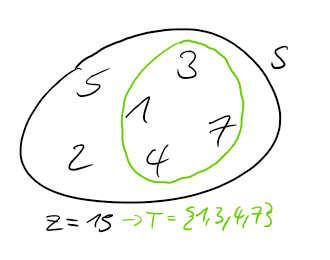
\includegraphics[scale=0.5]{./resources/teilmengen_summe.png}
\end{figure}
\textbf{Beweis}\\
\begin{itemize}
\item TMS $\in$ NP: T dient selbst als Zertifikat
\item NP-schwere zeigen durch Reduktion auf SAT
\begin{itemize}
\item Sei F eine KNF
\item seien $p_1, ..., p_n$ die Variablen in F
\item Definiere Gegenstände $t_i$ und $f_i$ für jede Variable $p_i$
\item die Kosten $v(t_i)$ und $v(f_i)$ seien also Binärfolge $a_1...a_n c_1...c_k$ gegeben
\begin{itemize}
\item die $a_i$'s kodieren die Variablen in 2er Potenzen
\item die $c_i$'s geben jeweils an ob die Variable $p_i$ für $t_i$ oder $\neq p_i$ für $f_i$ in der jeweiligen Disjunktion der KNF vorkommt
\end{itemize}
\item definiere ein $r = |C_i| - 1$
\item definiere die Menge S als $S = \{t_i f_i | 1 \leq i \leq n \} \cup \{m_{i,j} | 1 \leq i \leq k, 1 \leq j \leq |C_i| -1 \}$
\item z kann nun wie folgt bestimmt werden: $z=a_1...a_n c_1....c_k$ mit $a_i = 1$ und $c_i = |C_i|$
\item Die Teilmengen-Summe ist erfüllbar gdw. F erfüllbar ist
\begin{itemize}
\item Sei w eine erfüllende Belegung für F mit $w(p_i) = 1$ falls $t_i \in T$ und $w(p_i) = 0$ falls $f_i \in T$
\item definiere $T_1 = \{t_i | w(p_i) = 1, 1 \leq i \leq m \} \cup \{f_i | w(p_i) = 0, 1 \leq i \leq m \}$
\item definiere $T_2 = \{m_{i,j} | 1 \leq i \leq k, 1 \leq j \leq |C_i| - r_j \}$
\item die gesuchte Menge an Gegenständen ist $T = T_1 \cup T_2$
\end{itemize}
\item so folgt: $\sum_{s\in T} v(s) = z$
\item w ist wohldefiniert das $\forall i : t_i \in T \text{ xor } f_i \in T$
\end{itemize}
\end{itemize}
\begin{figure}[H]
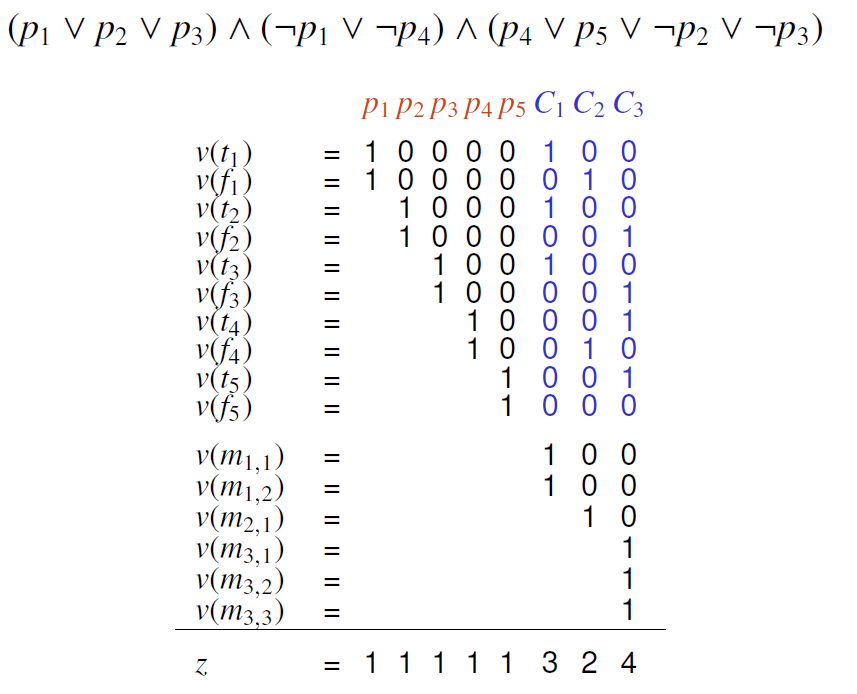
\includegraphics[scale=0.4]{./resources/TMS_beweis.png}
\end{figure}

\subsubsection{Nicht-Primzahl}
\textbf{Problem}
Sei eine natürliche Zahl $z>1$ gegeben. Gibt es eine $p,q>1$ mit $p\cdot q = z$ ? (Primfaktorzerlegung)

\subsubsection{Clique}
\textbf{Problem}\\
Sei ein Graph G und eine Zahl k gegeben. Enthält G eine vollvermaschte Knotenteilmenge mit k Knoten (Clique) ?
\textbf{Beweis}\\
\begin{itemize}
\item Clique $\in$ NP: Die Clique selbst ist ein Zertifikat
\item Clique ist NP-schwer. z.z. durch Reduktion auf SAT
\begin{itemize}
\item Sei F eine KNF
\item Sei $G_F$ ein Graph für den gilt: $G_F$ hat eine Clique der Größe l gdw. F erfüllbar ist
\item Knoten: Stehen in unterschiedlichen Disjunktionen der KNF, jeweils ein Paar aus Atom und Index der Disjunktion innerhalb der KNF
\item Kannten: zwischen Paaren, für welche der Index der Paares unterschiedlich ist und die Konjunktion der Atome erfüllbar ist
\end{itemize}
\item $G_F$ kann in PTime berechnet werden
\end{itemize}

\subsubsection{Rucksackproblem}
\textbf{Problem}
Sei G eine Menge von Gegenständen $a_1,...,a_n$ mit je einem Wert $v(a_i)$ und einem Gewicht $g(a_i)$.\\
Sei zudem w ein Mindestwert und l ein Gewichtslimit\\
Gibt es eine Teilmenge, der Gegenstände, welche das Gewichtslimit einhalten und trotzdem den Mindestwert erreichen ?\\

\textbf{Beweis}
\begin{itemize}
\item Rucksackproblem $\in$ NP: Zertifikat ist die gewählte Teilmenge
\item Rucksackprobem ist NP-schwer
\begin{itemize}
\item Reduktion des Rucksackproblems auf Teilmengen-Summe
\item Nehme eine Instanz des Teilmengen-Summe Problems mit $S = \{a_1,...,a_n$ und Wert $v(a_i)$, Wunschwert z
\item Setzte für alle Gegenstände $i\in G$ den Wert gleich dem Gewicht
\item Setze den Mindestwert w und das Maximalgewicht l gleich dem Wunschwert z
\item diese Übersetzung ist in PTime
\item somit gilt: $\sum_{vi\in T} v(a_i) = z$ gdw.\\
$\sum_{i\in T} v(i) \geq w = z$ und $\sum_{i\in T} g(i) \geq l = z$
\end{itemize}
\item $\rightarrow$ Das Rucksackproblem ist NP-vollständig
\end{itemize}

\subsection{Pseudopolynomielle Probleme}

\begin{itemize}
\item Ein Problem ist in pseudopolynomieller Zeit lösbar, wenn es von einer DTM gelöst wird welche polynomiell Zeitbeschränkt ist bzgl. der Eingabe \textbf{und} des Betrages aller zahlen in der Eingabe
\item oder: pseudopolynomieller wenn es in PTime liegt und alle Zahlen unär kodiert sind
\item durch pseudopolynomielle Zeit kann es so scheinen, als ob das Problem im PTime lösbar ist, ist es aber nicht
\item durch ineffiziente Kodierung der Eingabe wird so viel Platz geschaffen, dass ein Problem scheinbar in PTime lösbar wird\\da Resourcen nur im Bezug zur Inputgröße gemessen werden.
\item Beispiel: Input 1 Mrd = 1.000.000.000 $\rightarrow$ nur 10 Stellen aber eig. exponentiell Größer $10^9$\\
$\Rightarrow$ Kodierung lässt Wert klein aussehen
\item durch den übergroßen Input steht mehr Zeit zur Verfügung um das Problem scheinbar in PTime zu lösen
\end{itemize}
Note: Ist selbst nach einer unärkodierung ein Problem immer noch NP-vollständig, so heißt es \textbf{stark NP-vollständig}


\subsection{PSpace}
Es wird angenommen, dass Probleme in PSpace schwerer sind als NP

\subsubsection{Quantifizierte Boolsche Formel (QBF)}
\begin{itemize}
\item Eine QBF ist eine logische Formel, in welcher die Atome zusätzlich quantifiziert sind
\item z.B. $\forall p_1 \forall p_2 \exists p_2. (p_1 \land p_2) \lor (p_3 \rightarrow p_1)$
\item aufeinanderfolgende Quantoren können zusammengefasst werden:\\
$\forall p_1 \forall p_2$ = $\forall p_1, p_2$
\item $\phi [p/q]$ bedeutet $\phi$ mit p ersetzt durch q (im jeweiligen Scope)
\item \textbf{TrueQBF} ist das Problem ob $W(Q) = 1$
\item TrueQBF lässt sich auf SAT reduzieren, indem alle Quantoren Existenzquantoren werden
\item TrueQBF ist PSpace-vollständig
\begin{itemize}
\item TrueQBF $\in$ PSpace

\begin{itemize}
\item Sei F eine aussagenlogische Formel
\item enthält F keine Quantoren: löse F mit SAT
\item enthält F Existenzquantoren: 
\begin{itemize}
\item Teile die Formel auf
\item Teil 1: ersetze alle vorkommen der Quantifizierten Variable mit True
\item Teil 2: ersetzte alle vorkommen der Quantifizierten Variable mit False
\item Wende den Algorithmus rekursiv erneut auf Teil 1 und Teil 2 an
\item bilde die \textbf{Disjunktion} der beiden Ergebnisse
\end{itemize}
\item enthält F Allquantoren
\begin{itemize}
\item Teile die Formel auf
\item Teil 1: ersetze alle vorkommen der Quantifizierten Variable mit True
\item Teil 2: ersetzte alle vorkommen der Quantifizierten Variable mit False
\item Wende den Algorithmus rekursiv erneut auf Teil 1 und Teil 2 an
\item bilde die \textbf{Konjunktion} der beiden Ergebnisse
\end{itemize}
\end{itemize}
\end{itemize}
\item TrueQBF ist PSpace-schwer
\begin{itemize}
\item Darstellen des Laufes einer TM durch aussagenlogische Atome
\item Speicher ist wie bei NP polynomiell
\item Zeit kann in PSpace exponentiell sein, daher kann nicht einfach für jeden Zeitschritt eine neue Version der Konfiguration angelegt werden 
\item durchsuchen des exponentiell großen Graphen der TM durch \textbf{Middle-First-Search}
\begin{itemize}
\item Ziel: gelangt man von s nach t ?
\item Prüfe ob s = t oder s direkter Vorgänger von t
\item Rate einen Punkt m in der Mitte eines Pfades von s nach t (Raten erfordert NTM)
\item prüfe Rekursiv ob man von s nach m und von m nach t gelangen kann (wieder durch Raten)
\item Anzahl zu ratender Mittelpunkte ist logarithmisch zur Länge des Pfades\\
$\rightarrow$ somit braucht es durch logarithmisch viele Schritte in einem Exponentiellen Graph nur linear viele Schritte
\item Speicher kann in jedem Schritt wiederverwendet werden
\end{itemize}
\item der obrige Algorithmus lässt sich polynomiell in QBF kodieren
\end{itemize}
\end{itemize}
\begin{figure}[H]
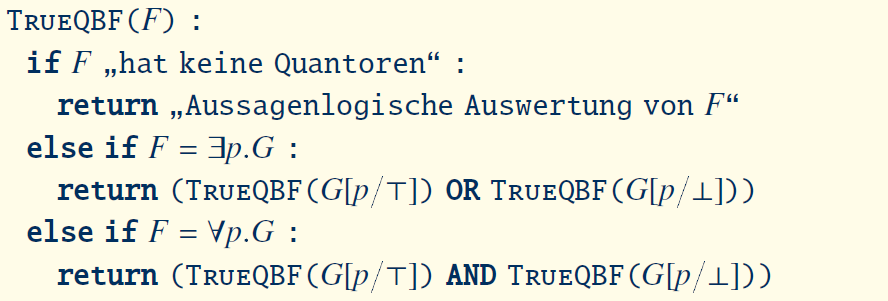
\includegraphics[scale=0.6]{./resources/QBF_algo.png}
\end{figure}

\subsection{Weitere Klassen}
\begin{itemize}
\item es lassen sich beliebig schwere Probleme der \textbf{k-Exp-Klasseen} konstruieren (k Höhe des Potenzturms)
\item es gibt Probleme jenseits der exponentiellen Klassen. Diese nennt man nicht-elementare Klassen
\item z.B. liegt Regex + Negationsoperator in dieser nicht-elementaren Klasse 
\end{itemize}

\section{Logik}

\subsection{Aussagenlogik}
\begin{itemize}
\item jedes Atom $p \in P$ ist eine aussagenlogische Formel
\item Seien F und G aussagenlogische Formeln, so sind es auch:
\begin{itemize}
\item Negation $\neg F$
\item Konjunktion $ F \land G $
\item Disjunktion $ F \lor G $
\item Implikation $ F \rightarrow G$
\item Äquivalenz $ F \leftrightarrow G $
\end{itemize}
\end{itemize}

\subsection{Prädikatenlogik}
\begin{itemize}
\item In der Prädikatenlogik benutzt man eine Art Methode (Prädikate) mit dem Returntype Bool um Aussagen zu tätigen
\item Die Prädikatenlogik ist \textbf{monoton}
\begin{itemize}
\item Je mehr Sätze es gibt desto weniger Modelle gibt es
\item Je mehr Sätze es gibt desto mehr Schlussfolgerungen kann man ziehen
\item Mehr Annahmen führen zu mehr Schlüssen
\end{itemize}
\begin{itemize}
\item Menge an Variablen V
\item Menge an Konstanten C
\item Menge and Prädikatensymbole P mit Stelligkeit $\geq$ 0
\end{itemize}
\item \textbf{Atom}: Ausdruck $p(t_1,...,t_n)$ für ein n-stelliges Prädikatensymbol\\
$p\in P$ und $t_i \in V \cup C$
\item die prädikatenlogischen Formeln sind wie die aussagenlogischen Formeln definiert mit dem Zusatz:
\item Existenzquantor $\exists x.F$
\item Allquantor $\forall x.F$
\end{itemize}

\subsubsection{Variablen}
\begin{itemize}
\item Alle Variablen in einem Atom sind frei
\item durch Verknüpfung ändert sich nichts an der 'Freiheit' einer Variable
\item eine Variable wird gebunden, wenn die im Bereich (Scope) eines Quantors auftaucht
\item Note: eine Variable kann gleichzeitig gebunden und frei auftauchen:\\
z.B. x in $p(x) \land \exists x.q(x)$
\item Formeln ohne freie Variablen heißen geschlossene Formeln oder \textbf{Sätze}
\item Formeln mit freien Variablen heißen offene Formeln
\item eine Menge von Sätzen nennt man auch \textbf{Theorie}
\end{itemize}

\subsubsection{Interpretation und Zuweisung}
Ersetzt die Wertzuweisung der Aussagenlogik
\textbf{Interpretation}
\begin{itemize}
\item $(\Delta^I, \times^I)$ Paar aus einer Domäne $\Delta^I$ und einer Interpretationsfunktion $\times^I$ 
\item die Interpretationsfunktion weißt jeder Konstante $a \in C$ ein Element der Domäne $a^I \in \Delta^I$ zu\\
$f(a) = a^I$
\item die Interpretationsfunktion weißt jedem n-stelligen Prädikatensymbol $p\in P$ eine Relation $p^I \subseteq (\Delta^I)^n$ zu\\
$f(p) = p^I$
\end{itemize}

\textbf{Zuweisung}
\begin{itemize}
\item Funktion welche einer Variable $x \in V$ eine Domänenelement $\delta \in \Delta^I$ zuweist
\item $Z[x \mapsto \delta]$ ist die Zuweisung, welche x auf $\delta$ und alle anderen Variablen auf $Z(y)$ abbildet
\end{itemize}

\textbf{Beispiel}
\begin{itemize}
\item Null ist eine natürliche Zahl, jede natürliche Zahl hat einen Nachfolger, dieser ist ebenfalls eine natürliche Zahl
\item $NatNum(null) \land \forall x. (NatNum(x) \rightarrow \exists y.(succ(x,y) \land NatNum(y)))$
\item Interpretation:
\begin{itemize}
\item $\Delta^I = \mathbb{R}$ (Menge der Reellen Zahlen)
\item $null^I = 0$ (definiert erste Zahl)
\item $NatNum^I = \mathbb{N} \subseteq \mathbb{R}$ (Menge der natürlichen Zahlen)
\item $succ^I \{(d,e) | d,e \in \mathbb{R}, d < e$ ($\rightarrow$ succ(2, 7) = 1, da 2 < 7)
\end{itemize}
\item es kann nun geschlussfolgert werden, dass NatNum(null) wahr ist, da $null^I \in NatNum^I$ gilt\\
$\rightarrow NatNum(num)^I = 1$
\item Zuweisung:
\begin{itemize}
\item Sei $Z(x)$ = 42
\item Sei $Z(y)$ = 5
\end{itemize}
\item Unter dieser Interpretation und Zuweisung ist das Atom $succ(x,y)$ falsch, da $(Z(x),Z(y) \not\in succ^I$ gilt (da 42 < 5 $\rightarrow$ Falsch $\rightarrow succ(x,y)^{I,Z} = 0$
\end{itemize}

\textbf{Atome Interpretieren}
\begin{itemize}
\item Sei I ein Interpretation
\item Sei Z eine Zuweisung für I
\begin{itemize}
\item Für eine Konstante c definieren wir $c^{I,Z} = c^I$
\item Für eine Variable x definieren wir $x^{I,Z} = Z(x)$
\end{itemize}
\item für ein Atom $p(t_1,...,t_n)$ setzten wir nun:
\begin{itemize}
\item $p(t_1,...,t_n)^{I,Z} = 1$ wenn $(t_1^{I,Z},...,t_n^{I,Z}) \in p^I$
\item $p(t_1,...,t_n)^{I,Z} = 0$ wenn $(t_1^{I,Z},...,t_n^{I,Z}) \not\in p^I$
\end{itemize}
\item Note: Interpretation wird hier auf 2 verschiedenen Ebenen benutzt!
\begin{itemize}
\item $t^{I,Z} \in \Delta1^I$ Interpretiert den Term
\item $A^{I,Z} \in \{0,1\}$ Interpretation von A und der Zuweisung Z ist Wahl/Falsch
\end{itemize}
\end{itemize}

\textbf{Formeln Interpretieren}
Eine Interpretation I und eine Zuweisung Z erfüllen eine Formel F ($I,Z \models F$) wenn gilt: 
\begin{tabular}{|c|c|c|}
\hline
Formel F & $I,Z \models F$ & $I,Z \not\models F$\\
\hline
F Atom & $F^{I,Z} = 1 $ & $ F^{I,Z} = 0$\\
\hline 
$\neg G$ & $I,Z \not\models G$ & $I,Z \models G$\\
\hline
$G_1 \land G_2$ & $I,Z \models G_1$ und $I,Z t\models G_2$ & $I,Z \not\models G$ oder $I,Z \not\models G$\\
\hline 
$G_1 \lor G_2$ & $I,Z \models G_1$ oder $I,Z \models G_2$ & $I,Z \not\models G$ und $I,Z \not\models G$\\
\hline 
$G_1 \rightarrow G_2$ & $I,Z \not\models G_1$ oder $I,Z \models G_2$ & $I,Z \models G$ und $I,Z \not\models G$\\
\hline 
$G_1 \leftrightarrow G_2$ & ($I,Z \models G_1$ und $I,Z t\models G_2$) oder ($I,Z \not\models G$ und $I,Z \not\models G$) & $\leftarrow$ -//- \\
\hline 
$\forall x.G$ & $I,Z[x\mapsto \delta] \models G, \forall \delta \in \Delta^I$ & $I,Z[x\mapsto \delta] \not\models G, \exists \delta \in \Delta^I$\\
\hline 
$\exists x.G$ & $I,Z[x\mapsto \delta] \models G, \exists \delta \in \Delta^I$ & $I,Z[x\mapsto \delta] \not\models G, \forall \delta \in \Delta^I$\\
\hline 
\end{tabular}

Eine Formel kann nach ihrem Modell
\begin{itemize}
\item allgemeingültig (tautologisch)
\item widersprüchlich (inkonsistent, unerfüllbar)
\item erfüllbar (konsistent)
\item widerlegbar
\end{itemize}
sein

\begin{figure}[H]
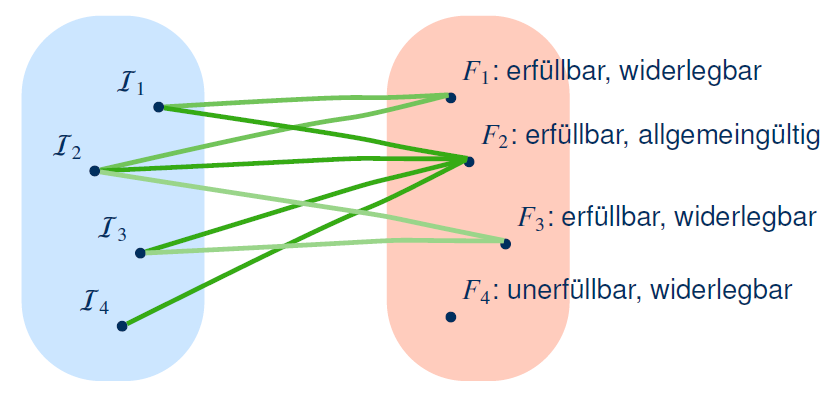
\includegraphics[scale=0.5]{./resources/model_types.png}
\end{figure}

\subsubsection{Logik auf Sätzen (Formeln ohne freie Variablen)}
Note: Eine Menge von Sätzen nennt man auch \textbf{Theorie}\\
ein Beispiel für eine Theorie ist z.B. die Theorie der partiellen Ordnung\\
\begin{itemize}
\item Sei I eine Interpretation und F eine Formel
\item Wenn $I \models F$ dann nennt man I ein Modell für F (I erfüllt F)
\item I ist ein Modell für eine Formelmenge (Theorie) T ($I \models T$) wenn $I \models F, \forall F\in T$
\item F ist eine logische Konsequenz aus einer Formel oder Formelmenge G ($G \models F$), wenn jedes Modell in G auch ein Modell von F ist ($I \models G \rightarrow G \models F$)\\ z.B. ist $I_1, I_2 \models F$ und $I_1 \models G$ dann $G \models F$
\item ist F eine Tautologie dann $\models F$ (ohne Voraussetzung gilt F)
\item Note: Alle Tautologien sind semantisch äquivalent, und in jedem Modell wahr, somit auch logische Konsequenz jeder Theorie
\item Zwei Formeln oder Formelmengen sind semantisch äquivalent $F \equiv G$, wenn sie die gleichen Modell haben\\
($I \models F \leftrightarrow I \models G, \forall I$) $\rightarrow$ (wechselseitige logische Konsequenz)
\end{itemize}

\subsubsection{Gleichheit und Ungleichheit}
\textbf{Definition}
\begin{itemize}
\item Gleichheit: $\approx^I = \{(\delta, \delta) | \delta \in \Delta^I\}$
\item meist infix geschrieben
\item Beispiel: $\forall x, y.(erde(x) \land erde(y) \rightarrow x \approx y)$ = es gibt nur eine Erde
\item Eigenschaften von $\approx$ logisch beschrieben:
\begin{itemize}
\item Reflexivität: $\forall x.eq(x,x)$
\item Symmetrie: $\forall x,y.eq(x,y) \rightarrow eq(y,x)$
\item Transitivität: $\forall x,y,z.eq(x,y) \land eq(y,z) \rightarrow eq(x,z)$
\item Kongruenz: $\forall x_1,...,x_n,y.((p(x_1,...,x_i,...,x_n) \land eq(x_i, y)) \rightarrow p(x_1,...,y,...,x_n))$\\
da $x_i = y$ können diese ausgetauscht werden (ersetze gleiches mit Gleichem)
\end{itemize}
\item Ungleichheit: $\forall x, y.(x \not\approx y \leftrightarrow \neg x \approx y)$
\end{itemize}

\textbf{Liste von Gleichheiten}
\begin{itemize}
\item $\neg \exists.F \equiv \forall x.\neg F$
\item $\neg \forall.F \equiv \exists x.\neg F$
\item $\exists x. \exists y.F \equiv \exists y. \exists x.F$
\item $\forall x. \forall y.F \equiv \forall y. \forall x.F$
\item $\exists x.(F \lor G) \equiv (\exists x.F \lor \exists x.G)$
\item $\forall x.(F\land G) \equiv (\forall x.F \land \forall x.G)$
\end{itemize}

\textbf{Liste von Ungleichheiten}
\begin{itemize}
\item $\exists x. \forall y.F \not\equiv \forall y. \exists x.F$\\
$\rightarrow$ (Jeder hat einen Vater $\neq$ Es gibt einen Vater aller)
\item $\forall x.(F\lor G) \equiv (\forall x.F \lor \forall x.G)$\\
$\rightarrow$ (Jeder ist entweder glücklich oder nicht $\neg$ es sind alle glücklich oder nicht)
\end{itemize}

\subsubsection{Unentscheidbarkeit}
Logisches schließen in der Prädikatenlogik ist unentscheidbar\\
Dies gilt auch wenn nur binäre Prädikatensymbole zugelassen sind\\
\textbf{Beweis}\\
\begin{itemize}
\item Reduktion des CFG-Schnittproblems
\begin{itemize}
\item Gegeben 2 kontextfreie Grammatiken (CFG) $G_1$ und $G_2$
\item Gibt es ein Wort $w \in L(G_1) \cap L(G_2)$ ?
\end{itemize}
\item kodieren von Wörtern als Kette von binären Relationen aus der Prädikatenlogik (für Terminale und nicht Terminale)
\begin{itemize}
\item Beispiel 'baum'
\begin{itemize}
\item $(\delta_0, \delta_1) \in p_b^I$
\item $(\delta_1, \delta_2) \in p_a^I$
\item $(\delta_2, \delta_3) \in p_u^I$
\item $(\delta_3, \delta_4) \in p_m^I$
\item = $\delta_0 \rightarrow^{p_b} \delta_1 \rightarrow^{p_a} \delta_2 \rightarrow^{p_u} \delta_3 \rightarrow^{p_m} \delta_4$
\end{itemize}
\end{itemize}
\item nehme an, dass $G_1$ und $G_2$ keine gemeinsamen nicht Terminale habe (Terminale schon)
\item kodiere jedes nicht Terminal $A \rightarrow \sigma_1\cdots\sigma_n$ als Formel
\item konstruiere eine Formel, welche erkennt ob eine Folge von Terminalen und nicht Terminalen aus einem anderen nicht Terminal entstehen kann\\
($\beta = \alpha_1\cdots\alpha_n, \alpha_i \in T\cup N, \beta \in N$)\\
erkennt ob eine Zeichenkette aus einem anderen nicht Terminal abgeleitet werden kann
\item Formel: $\forall x_0,...,x_n.((p_{\sigma_1}(x_0,x_1)\land \cdots \land p_{\sigma_n}(x_{n-1},x_n)) \rightarrow p_A(x_0,x_n))$ gibt es eine Kette in Modell, dann verbinde deren erstes und letztes Symbol mit einem $p_A$ (A ist nicht Terminal)
\item Seien $S_1$ und $S_2$ die Startsymbole von $G_1$ und $G_2$
\item kodiere das Schnittproblem wie folgt:
\begin{itemize}
\item $\exists x,y.(p_{S_1}(x,y) \land p_{S_2}(x,y))$
\item gibt es ein Modell ohne Zyklen oder parallele Relationen welches die obrige Formel erfüllt, so muss es ein Wort geben, welches im Schnitt der Sprachen liegt
\end{itemize}
\item es müssen noch alle möglichen Wörter kodiert werden, dafür
\begin{itemize}
\item $\forall x. \exists y.p_a(x,y), \forall a\in T$
\end{itemize}
\item konstruiere eine Theorie TH aus $G_1$ und $G_2$
\item dann muss gelten: $TH \models \exists x,y.(p_{S_1}(x,y) \land p_{S_2}(x,y))$ gdw. $w\in L(G_1) \cap L(G_2)$ gilt
\end{itemize}

\subsection{Negations Normal Form (NNF)}
eine Formel F ist in NNF wenn:
\begin{itemize}
\item enthält nur Quantoren und die Junktoren \textbf{und} ($\land$), \textbf{or} ($\lor$), \textbf{not} ($\lnot$)
\item der Junktor $\lnot$ kommt nur direkt vor einem Atom vor
\end{itemize}
\textbf{Umwandlung}
\begin{itemize}
\item ersetze $F \rightarrow G$ durch $\lnot F \lor G$
\item ersetze $G \leftrightarrow G$ durch $(\lnot F \lor G) \land (\lnot G \lor F)$
\end{itemize}

\subsection{Bereinigte Formel}
eine Formel F ist bereinigt wenn:
\begin{itemize}
\item keine Variable in F gleichzeitig gebunden und frei vorkommt
\item keine Variable in F von mehr als einem Quantor gebunden wird
\end{itemize}
\textbf{Umwandlung}
\begin{itemize}
\item entfernen von Quantoren die nichts binden (x kommt in F nicht als freie Variable vor)
\begin{itemize}
\item $\exists x.F \equiv F \equiv \forall x.F$
\item $\exists x. (F\land G) \equiv (F \land \exists x.G) \equiv (\exists x.F \land \exists x.G)$
\item $\forall x. (F \lor G) \equiv (F \lor \forall x.G) \equiv (\forall x.F \lor \forall x.G)$
\item $\exists x. \forall y.F \equiv \forall y .\exists x .F$
\item $\forall x . \exists y .F \equiv \exists y .\forall x .F$
\end{itemize}
\item Variablenumbenennung
\begin{itemize}
\item Eine Variable kann umbenannt werden, sofern dies die Semantik der Formel nicht verändert
\item $Qx.F \equiv Qy.F\{x\mapsto y\}$ mit $Q \in \{ \forall, \exists \}$, wenn y nicht in F vorkommt
\end{itemize}
\end{itemize}

\subsection{Pränexform}
Eine Formel F ist in Pränexform wenn alle Quantoren am \textbf{Anfang} stehen\\
$Q_1x_1.\cdots Q_nx_n.F, Q\in\{ \forall ,\exists \}$\\
\textbf{Umwandlung}\\
\begin{itemize}
\item Sei F eine bereinigte Formel in NNF
\item $Qx.F \circ G) \mapsto Qx.(F\circ G)$
\item $(G \circ Qx.F) \mapsto Qx.(G\circ F)$
\item $Q \in \{ \forall, \exists \}$, $\circ \in \{ \land ,\lor \}$
\end{itemize}

\subsection{Skolemisierung}
Einführen von Funktionssymbolen in die Logik\\
\textbf{Umwandlung}
\begin{itemize}
\item Sei $\forall x_1.\cdots\forall x_n.\exists y.F$ eine Formel in Pränexform
\item Die Skolemisierung von y ist die Formel $\forall x_1.\cdots\forall x_n.F'$
\begin{itemize}
\item $F' = F\{y\mapsto f(x_1,...,x_n)\}$ ersetze jedes freie Vorkommen von y in F durch $f(x_1,...,x_n)$
\item die Funktion f muss dabei 'neu' sein und darf nirgends sonnst bisher vorkommen
\end{itemize}
\item führe die obrige Umformung für jede existenziell quantifizierte Variable (mit $\exists$), von vorn nach hinten durch
\end{itemize}
\textbf{Beispiel}
\begin{itemize}
\item $\forall x.\exists y. \forall z. \exists v.p(x,y,z,v)$
\item Skolemisiere y: = $\forall x.\forall z.\exists v.p(x,f(x),z,v)$ (y wird zu f(x), da y von x allquantifiziert wird)
\item Skolemisiere v: = $\forall x. \forall z.p(x,f(x),z,g(x,z))$ (v wird zu g(x,z), da v von x und z allquantifiziert wird)
\end{itemize}

\subsection{Konjunktive Normalform (KNF)}
Eine Formel F ist in KNF wenn:
\begin{itemize}
\item sie in Pränexform ist
\item die Form $(L_{1,1} \lor \cdots \lor L_{1,m}) \land (L_{n,1} \lor \cdots \lor L_{n,m})$ hat
\item L sind Literale
\item Klauseln sind Disjunktionen ($\lor$) von Literalen
\end{itemize}
\textbf{Umwandlung}
\begin{itemize}
\item $F \lor (G \land H) \mapsto (F\lor G) \land (F \lor H)$
\end{itemize}



\subsection{Unifikation}
\subsubsection{Substitution}
\begin{itemize}
\item Menge von Ersetzungsregeln
\item $\{x_1\mapsto t_1,...,x_n\mapsto t_n\}$
\item $x_i \in V$ paarweise verschieden, $t_i\in T$ beliebige Terme
\item Komposition von Substitutionen (Hintereinanderausführung)
\begin{itemize}
\item Komposition $\sigma \circ \theta$
\item $\sigma = \{x_1\mapsto t_1,...,x_n\mapsto t_n\}$, $\theta = \{y_1\mapsto s_1,...,y_m\mapsto s_m\}$
\item $\sigma \circ \theta = \{x_1\mapsto t_1 \theta ,...,x_n \mapsto t_n \theta \} \cup $\\
$\{ y_i \mapsto s_i \vert y_i \in 
\{ y_1,...,y_m \} \setminus \{x_1,...,x_n \} \}$
\end{itemize}
\end{itemize}

\textbf{Unifikator}\\
\begin{itemize}
\item Sei G eine Menge von Gleichungen der Form $G = \{ s_1 = t_1, ..., s_n = t_n \}$
\item Ein Unifikator ist eine Substitution $\sigma$ für welche $s_i\sigma = t_i\sigma, \forall i\in \{1,...,n\}$ gilt
\item ein Unifikator ist also eine Menge von Überführungsregeln um eine Menge von Gleichungen syntaktisch anzugleichen
\item Beispiele
\begin{itemize}
\item $\{f(x) = f(y)\}$ hat den Unifikator $\{x\mapsto y\}$
\item $\{f(x) = g(x) \}$ hat keinen Unifikator
\end{itemize} 
\item Es gibt einen allgemeinsten Unifikator (most general unifier (mgu))
\begin{itemize}
\item Eine Substitution $\sigma$ ist allgemeiner als eine Substitution $\theta$ ($\sigma \preceq \theta$) wenn:
\begin{itemize}
\item es eine Substitution $\lambda$ gibt, sodass $\sigma \circ \lambda = \theta$
\item ein allgemeiner Unifikator kann also erhalten werden, indem eine Teilmenge ($\lambda$) von ihm abgespalten wird
\item daraus folgt auch, dass der MGU nicht weiter zerlegt werden kann
\end{itemize}
\end{itemize}
\item \textbf{Unifikationsalgorithmus}
\begin{itemize}
\item Sei G ein Unifikationsproblem
\item \textbf{Löschen}: $\{t = t\} \cup G' \rightarrow G$\\
 syntaktisch gleiche Gleichungen können aus G entfernt werden
\item \textbf{Zerlegung/Dekomposition}: $\{f(s_1,...,s_n) = f(u_1,...,u_n)\} \cup G' \rightarrow \{s_1 = u_1,...,s_n=u_n\} \cup G'$\\
wird die gleiche Funktion auf eine Anzahl von Variablen angewendet, so kann man die Funktion weglassen
\item \textbf{Orientierung}: $\{t=x\} \cup G' \rightarrow \{ x=t\} \cup G'$ mit $x\in V$ und $t\not\in V$\\
Kommutativität
\item \textbf{Eleminierung}: $\{x=t\} \cup G' \rightarrow \{x=t\} \cup G'\{x\mapsto t\}$, für $x\in V$ und $x \not\in t$\\
Einsetzten in die anderen Gleichung, das Eingesetzte verschwindet dabei
\end{itemize}
\end{itemize}
\begin{figure}[H]
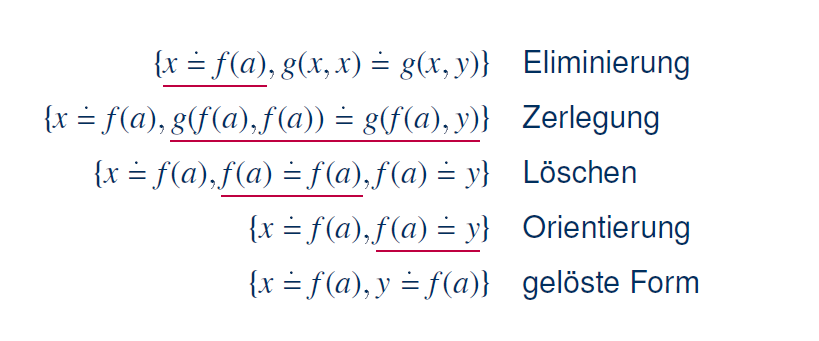
\includegraphics[scale=0.5]{./resources/uni_bsp.png}
\end{figure}

\textbf{Beweis der Korrektheit}
Der Unifikationsalgorithmus liefert immer den MGU oder nicht-unifizierbar
\begin{itemize}
\item Hilfsaussage $\bigstar$: Wenn ein Unifikationsproblem $G_1$ in eimem Eretzungschritt in ein Problem $G_2$ umgewandelt werden kann, dann haben $G_1$ und $G_2$ die gleichen Unifikatoren
\begin{itemize}
\item für Löschen, Orientierung, Zerlegung trivial
\item für Eleminierung
\begin{itemize}
\item Sei $G_1 = \{ x=t\} \cup G'$ und $\sigma = \{ x\mapsto t \}$
\item dann ist $G_2 = \{x=t\} \cup G'\sigma$
\item Sei $\theta$ Unifikator für $G_1$, 
\item gdw. $x\theta = t\theta$ und $\theta$ Unifikator für G'
\item gwd. $x\theta = t\theta$ und $\sigma\circ\theta$ Unifikator für G', da $\sigma = \sigma_{\{x=t\}}$ und so $\theta = \sigma \circ \theta$ für alle Unifikatoren von $\theta$ von $\{x=t\}$
\item gdw. $x\theta = t\theta$ und $\theta$ Unifikator für $G'\sigma$
\item gdw. $\theta$ Unifikator für $\{x=t\} \cup G'\sigma = G_2$
\end{itemize}
\end{itemize}
\item Wenn der Algorithmus eine Substitution $\sigma$ liefert, dann ist $\sigma$ MGU
\begin{itemize}
\item nach $\bigstar$ erhält jeder Umformungsschritt die Unifikatoren, somit auch die allgemeinsten Unifikatoren
\item Per Induktion gilt, dass jedes Unifikationsproblem, welches der Algorithmus erzeugt, hat den gleichen MGU wie G hat
\item Wenn der Algorithmus also einen Unifikator zurückgibt, ist dieser der MGU
\end{itemize}
\item Wenn der Algorithmus nicht-unifizierbar liefert, dann hat G keinen Unifikator
\begin{itemize}
\item sollte es keinen Unifikator geben, so muss das Problem G' eine der folgenden Gleichungen enthalten
\begin{itemize}
\item x = t, mit $x\in V$ und $x\in t$
\item $f(\cdots) = g(\cdots)$ mit $f\neq g$
\end{itemize}
\item Fall 1: $s=u$ hat auf einer Seite eine Variable. Dann hat sie Form 1, da sonst Orientierung oder Löschen möglich wäre
\item Fall 2: $s=u$ hat auf keiner Seite eine Variable. Dann hat sie Form 2, da sonst Zerlegung möglich wäre
\end{itemize}
\item Der Algorithmus terminiert nach endlich vielen Schritten
\begin{itemize}
\item anordnen des Unifikationsproblems so, dass das Problem in jedem Schritt kleiner wird
\item Sei v die Anzahl nicht gelöster Variablen in G'
\item Sei g die Gesamtzahl (Summe) der Vorkommen von Funktionssymbolen, Konstanten und Variablen in G
\item Sei r die Anzahl der Gleichung in $s=x \in G'$ mit $x\in V$ auf der \textbf{rechten} Seite
\item ordne nun das Problem G' lexikographisch bzgl. der Tripel $\kappa(G')$
\item Für $G_1$ und $G_2$ mit $\kappa(G') = (v_i, g_i, r_i)$ gilt $G_1 \prec G_2$ falls min eines davon gilt:
\begin{itemize}
\item $v_1 > v_2$
\item $v_1 = v_2$ und $g_1 > g_2$
\item $v_1 = v_2$ und $g_1 = g_2$ und $r_1 > r_2$ 
\item man vergleicht immer die Stellen im Tripel und hört auf zu vergleichen wenn etwas nicht gleich ist
\item Beispiel: $(4, 2, 1) \prec (3, 42, 23) \prec (3, 42, 22) \prec (3, 41, 1000)$
\end{itemize}
\item Die Behauptung folgt nun, da jede Regelanwendung zu einem kleineren ($\prec$) Unifikationsproblem führt
\item Da es keine unendlichen Ketten immer kleiner werdender Probleme gibt muss der Algorithmus terminieren
\end{itemize}
\end{itemize}
\begin{figure}[H]
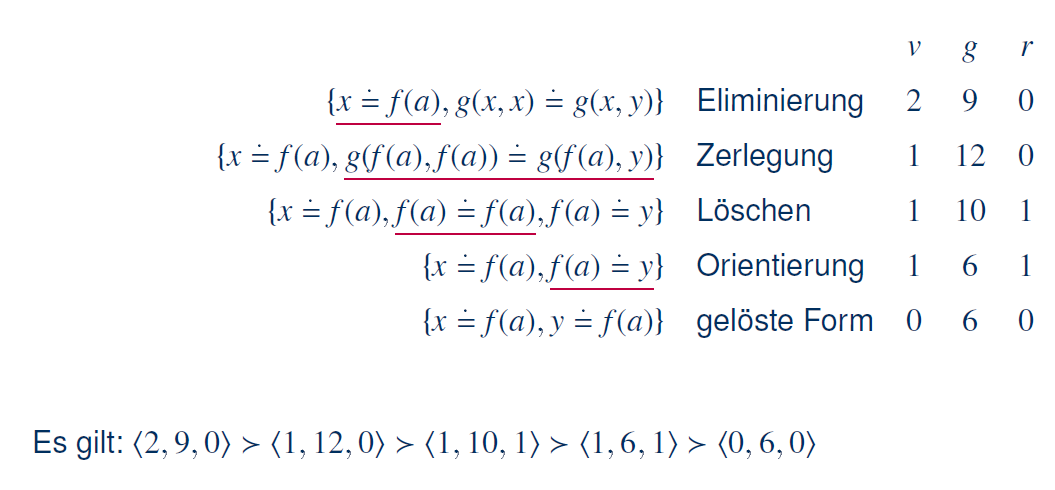
\includegraphics[scale=0.5]{./resources/uni_term.png}
\end{figure}

\subsection{Resolution}
\subsubsection{Resolvente}
\begin{itemize}
\item Sei $K_1 = \{A_1,...,A_n, L_1,...,L_k \}$ und $K_2 = \{\lnot A_1',...,\lnot A_m',L_1',...,L_l' \}$ Klauseln
\item Sei $\sigma$ der MGU der Menge $\{A_1,...,A_n,A_1',...,A_m' \}$
\item Seien $L_i$ und $L_j'$ beliebige Literale
\item die Resolvente ist nun die Klausel der Form $\{L_1 \sigma,...,L_k \sigma , L_1' \sigma,...,L_l' \sigma \}$
\item in der Resolvente löschen sich also immer zwei entgegengesetzte Teilterme aus
\item führt man die Resolution immer wieder aus und erhält die leere Menge so ist die Formel erfüllbar
\item erhält man die leere Menge nicht, so ist die Formel unerfüllbar
\end{itemize}

\subsection{Herbrantmodelle}
Ziel: \textbf{Semantik aus Syntax}:\\
Konstruktion von Modellen direkt aus den Formeln, welche sie erfüllen sollen

\textbf{Herbrantuniversum}
\begin{itemize}
\item Sei $\Delta_F$ das Herbrantuniversum für eine Formel F
\item die Menge aller Terme ohne Variablen die man mit Konstanten und Funktionssymbolen in F und einer zusätzlichen Konstante a bilden kann
\begin{itemize}
\item $a \in \Delta_F$ (per Definition)
\item $c \in \Delta_F$ für jede Konstante aus F
\item $f(t_1,...,t_n \in \Delta_F$ für jedes n-stellige Funktionssymbol in F und alle Terme $t_1,...t_n \in \Delta_F$
\end{itemize}
\item Note: Das Herbranduniversum ist immer abzählbar, nicht aber zwingend endlich
\item Beispiel:
\begin{itemize}
\item $F = p(f(x),y,g(z))$
\item $\Delta_F = \{a, f(a), g(a), f(f(a)), f(g(a)), g(f(a)), g(g(a)),... \}$
\end{itemize}
\end{itemize}

\textbf{Herbrantinterpretation}
\begin{itemize}
\item Ist die Interpretation I für F für welche gilt: $\Delta^I = \Delta_F$
\item für jeden Term $t \in \Delta_F$ gilt $t^I = t$
\item Ist I ein Modell für F ($I \models F$), dann ist I ein \textbf{Herbrandmodell} für F
\item Es ist egal ob eine Ersetzung auf eine Zuweisung oder eine Formel angewendet wird:
\item $I,Z\{x\mapsto t\} \models F$ gdw. $I,Z \models F\{x\mapsto t\}$
\item Ein Satz F in Skolenform ist erfüllbar gdw. F ein Herbrandmodell ist
\end{itemize}

\textbf{Beispiele}
\begin{itemize}
\item $I_1$ mit $hatVater^{I_1}$ = $\emptyset$ kein Herbrandmodell, Formel nicht erfüllt (niemand hat einen Vater)
\item $I_2$ mit $hatVater^{I_2}$ = $\{(t,(f(t) | t \in \Delta_F \}$ Herbrandmodell, da Formel erfüllt
\item $I_3$ mit $hatVater^{I_3}$ = $\Delta_F \times \Delta_F$ Herbrandmodell, da Formel erfüllt
\end{itemize}


\end{document}